\documentclass{easyclass}

\usepackage{todonotes}
\usepackage{mathtools}
\usepackage{cancel}
\usepackage{xfrac}
\usepackage{float}
\usepackage{caption}

\begin{document}
\begin{titlepage}
    \university{Politicnico di Milano}
    \courseid{MIDA2}
    \title{Model Identification and Data Analysis \par Part 2}
    \author{Marco Donadoni and Edoardo Morassutto}
    \version{2019 -- 2020}
    \instructor{Instructors:\par Prof. \textsc{Sergio Savaresi}\par
    Ing. \textsc{Stefano Dattilo}}
    \maketitle
\end{titlepage}

\tableofcontents

%\input{lectures/template.tex}
\section{Table}

\begin{table}[htp]
    \centering
    \begin{tabular}{r|l|p{10cm}}
        Right &  Left  &  Longlonglonglonglonglonglonglong longlonglonglonglonglonglonglonglonglonglonglonglong longlonglonglonglonglong \\
        Right &  Left  &  Longlonglonglonglonglonglong
        longlonglonglonglonglonglonglong
        longlonglonglong
        longlonglonglonglonglonglonglong
    \end{tabular}
    \caption{This is a caption}
    \label{tab:trans-sym}
\end{table}

\section{List}
This is a List:
\begin{itemize}
    \item \textbf{Bullet 1}: Bullet 1 is bullet 1.
    \item \textbf{Bullet 2}: Bullet 2 is bullet 2.
\end{itemize}

\section{Definition}
\begin{definition}\label{def:def1}
\textbf{DEFINITION NAME}: This is a definition.
\end{definition}

% avoid bad break
\vspace{5cm}

\section{Theorem}
\begin{theo}[THEOREM NAME]{theo:theo1}
This is a theorm. Below are equations.
\begin{align}\label{eq:multi-equations}
    \psi(\bvec{a}) &= A\cdot \bvec{a} + \bvec{t}.\\
    R_x &=  \begin{bmatrix}
            0 & \cos(\theta) & -\sin(\theta)\\
            0 & \sin(\theta) & \cos(\theta)\\
            1 & 0 & 0
         \end{bmatrix},
    R_y =  \begin{bmatrix}
            \cos(\theta) & 0 & -\sin(\theta)\\
            \sin(\theta) & 0 & \cos(\theta)\\
            0 & 1 & 0
         \end{bmatrix},
    R_z =  \begin{bmatrix}
            \cos(\theta) & -\sin(\theta) & 0\\
            \sin(\theta) & \cos(\theta) & 0 \\
            0 & 0 & 1
         \end{bmatrix}
\end{align}
\end{theo}

\begin{lem}[LEMMA NAME]{lem:leml}
This is a lemma
\end{lem}

\begin{prf}[LEMMA NAME]{prf:leml}
This is a proof.
\end{prf}

\section{Tikz Pictures}
\begin{figure}[htp]
    \centering
        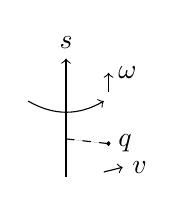
\begin{tikzpicture}[scale=0.6]
            \draw[->] (0,-1)--(0,1.5)node[above] {$s$};
            \draw[->] (-0.8,0.6) to[bend right] (0.8,0.6);
            \draw[->] (0.9, 0.8)--(0.9, 1.2) node[right] {$\omega$};
            \filldraw[dashed] (0,-0.2)--(0.9, -0.3) circle (1pt) node [right] {$q$};
            \draw[->] (0.8, -0.9)--(1.2, -0.8) node[right] {$v$};
        \end{tikzpicture}
    \caption{This is a caption. }
    \label{fig:rotation}
\end{figure}





\curinstructor{Ins Tructor1}

\begin{remark}[Strictly proper systems]
    Notice that for strictly proper systems the delay $k \ge 1$
\end{remark}
\missingfigure{Graphs about strictly proper systems}

\subsection{Representation \#3: convolution of the input with the Impulse Response (IR)}
The third way to represent a system is through the convolution of the input with the \emph{Impulse Response (IR)}.
\missingfigure{Graphs about convolution}
It can be proven that the input-output relationship from $u(t)$ to $y(t)$ can be written as
\[ y(t) = \omega(0) u(t) + \omega(1) u(t-1) + \omega(2) u(t-2) + \cdots \]
It can be rewritten as follows
\[ y(t) = \sum_{k=0}^{\infty} \omega(k) u(t-k) \]
From this, it is clear that $y(t)$ is the convolution of IR with the input signal.
\missingfigure{Block diagram of system}

\section{Transformation between representations}
\missingfigure{Figure of translation between representations}
\subsection{State Space to Transfer function}
Consider a strictly proper system with the following state space representation:
\[
\begin{cases}
    x(t+1) = F x(t) + G u(t)\\
    y(t) = H x(t) + \cancelto{0}{D u(t)}\\
\end{cases}
\Rightarrow
\begin{cases}
    x(t+1) = F x(t) + G u(t)\\
    y(t) = H x(t)\\
\end{cases}
\]
From the system we get
\[ z x(t) = F x(t) + G u(t) \Rightarrow x(t) = (zI - F)^{-1} G u(t) \]
\[ \Rightarrow y(t) = H (zI - F)^{-1} G \cdot u(t) \]
Thus, the transfer function is
\[ W(z) = H(zI - F) ^ {-1} G \]

\begin{example}
\begin{align*}
    F = \begin{bmatrix}
        1 & 0\\
        \frac{1}{2} & 2\\
    \end{bmatrix}
    &&
    G = \begin{bmatrix}
        1\\
        1\\
    \end{bmatrix}
    &&
    H = \begin{bmatrix}
        1 & 0\\
    \end{bmatrix}
    &&
    D = 0
\end{align*}
\begin{align*}
W(z) &=
\begin{bmatrix}
    1 & 0\\
\end{bmatrix}
\left( \begin{bmatrix}
    z & 0\\
    0 & z\\
\end{bmatrix}
-
\begin{bmatrix}
    1 & 0 \\
    \frac{1}{2} & 2\\
\end{bmatrix}\right)^{-1}
\begin{bmatrix}
    1\\
    1\\
\end{bmatrix}
= \begin{bmatrix}
    1 & 0\\
\end{bmatrix}
\begin{bmatrix}
    z-1 & 0\\
    -\frac{1}{2} & z-2\\
\end{bmatrix}^{-1}
\begin{bmatrix}
    1\\
    1\\
\end{bmatrix}\\
&= \begin{bmatrix}
    1 & 0\\
\end{bmatrix}
\frac{1}{(z-1)(z-2)}
\begin{bmatrix}
    z-2 & 0\\
    \frac{1}{2} & z-1\\
\end{bmatrix}
\begin{bmatrix}
    1\\
    1\\
\end{bmatrix}
=
\frac{1}{(z-1)(z-2)}
\begin{bmatrix}
    z-2 & 0\\
\end{bmatrix}
\begin{bmatrix}
    1\\
    1\\
\end{bmatrix}\\
&=
\frac{\cancel{z-2}}{(z-1)\cancel{(z-2)}} = \frac{1}{z-1} = \frac{1}{1-z^{-1}} z^{-1}
\end{align*}
Notice that in this case we only have one pole, but the system is of order two; this comes from the fact that part of the system is non observable.

\end{example}

\subsection{Transfer function to State Space}
This conversion is not very used in practice and it is called the \emph{realization} of a transfer function into a state space model.

Note that the state space representation is not unique, so from a single transfer function we can get infinite different equivalent state space models.

\begin{example}[Control realization]

We assume that the system is strictly proper and that the denominator is monic.
\[ W(z) = \frac{b_0 z^{n-1} + b_1 z^{n-2} + \dots + b_{n-1}}{z^n + a_1 z^{n-1} + a_2 z^{n-2} + \dots + a_n} \]

The formula for the control realization of $W(z)$ is
\begin{align*}
    F = \begin{bmatrix}
        0 & 1 & 0 & \cdots & 0\\
        0& 0 & 1 & \ddots & \vdots \\
        \vdots & \vdots & \ddots & \ddots & 0\\
        0 & 0 & \cdots & 0 & 1\\
        -a_n & -a_{n-1} & \multicolumn{2}{c}{\cdots} & -a_1\\
    \end{bmatrix}
    &&
    G = \begin{bmatrix}
        0\\
        0\\
        0\\
        \vdots\\
        1\\
    \end{bmatrix}
    &&
    H = \begin{bmatrix}
        b_{n-1} & b_{n-2} & \cdots & b_0\\
    \end{bmatrix}
    &&
    D = 0
\end{align*}
\end{example}

\newpage
\newlecture{Sergio Savaresi}{21/04/2020}

\begin{figure}[H]
    \centering
    \begin{tikzpicture}[node distance=2.5cm,auto,>=latex']
        \node (n1) {\#1};
        \node (n2) [below of=n1, xshift=-1.8cm] {\#2};
        \node (n3) [below of=n1, xshift= 1.8cm] {\#3};

        \draw[->] (n1) edge[bend right] (n2);
        \draw[->] (n2) edge[bend right] (n3);
        \draw[->] (n1) edge[bend left] (n3);
        \draw[->, dashed] (n2) edge[bend right=20] (n1);
        \draw[->, dotted] (n3) edge[bend right=20] (n2);
        \draw[->, dashed, red] (n3) edge[bend left=20] node {?} (n1);
    \end{tikzpicture}
\end{figure}

\section{Fundamental concepts of observability and controllability}

\[
    \begin{cases}
        x(t+1) = Fx(t) + Gu(t) \\
        y(t) = Hx(t)
    \end{cases}
\]

\subsection{Fully Observable}
The system is fully observable (from the output) if and only if the observability matrix is full rank:
\[
    O = \begin{bmatrix}
        H \\
        HF \\
        \vdots \\
        HF^{n-1}
    \end{bmatrix}
    \qquad
    \rank O = n
\]

\subsection{Fully Controllable}
The system is fully controllable (from the input) if and only if the controllability matrix is full rank:
\[
    R = \begin{bmatrix}
        G & FG & \cdots & F^{n-1}G
    \end{bmatrix}
    \qquad
    \rank R = n
\]

$R$ is also called \emph{reachability} matrix.

\begin{remark}
    \begin{description}
        \item[Observability] we can observe the state from the output sensors.
        \item[Controllability] we can control/move/influence the state using the input signal.
    \end{description}
\end{remark}

\begin{example}
    \begin{align*}
        \begin{cases}
            x_1(t+1) = \frac{1}{2} x_1(t) + u(t) \\
            x_2(t+1) = \frac{1}{3}x_2(t) \\
            y(t) = \frac{1}{4}x_1(t)
        \end{cases}
        \qquad
        F = \begin{bmatrix}
            \frac{1}{2} & 0 \\
            0 & \frac{1}{3}
        \end{bmatrix}
        \qquad
        H = \begin{bmatrix}
            \frac{1}{4} & 0
        \end{bmatrix}
        \qquad
        G = \begin{bmatrix}
            0 \\
            1
        \end{bmatrix}
    \end{align*}

    \[
        O = \begin{bmatrix}
            H \\
            HF
        \end{bmatrix} = \begin{bmatrix}
            \frac{1}{4} & 0 \\
            \frac{1}{8} & 0
        \end{bmatrix}
        \qquad
        \rank O = 1 < n = 2
        \quad\implies\quad \text{not fully observable}
    \]

    \[
        R = \begin{bmatrix}
            G & FG
        \end{bmatrix} = \begin{bmatrix}
            0 & 0 \\
            1 & \frac{1}{3}
        \end{bmatrix}
        \qquad
        \rank R = 1 < n = 2
        \quad\implies\quad \text{not fully controllable}
    \]
\end{example}

\begin{remark}[4 sub-systems]
    Each system can be internally seen as 4 sub-systems as follows:

    \begin{figure}[H]
        \centering
        \begin{tikzpicture}[node distance=1.5cm,auto,>=latex']
            \node[int, align=center] (noc) {NO\\C};
            \node[int, align=center, below of=noc] (onc) {O\\NC};
            \node[int, align=center, below of=onc] (oc) {O\\C};
            \node[int, align=center, below of=oc] (nonc) {NO\\NC};

            \node at (-5cm,-1.5cm) (u) {$u$};
            \node[coordinate] at (-3cm,-1.5cm) (input) {};
            \node at (5cm,-2.5cm) (y) {$y$};
            \node[coordinate] at (3cm,-2.5cm) (output) {};
            \node[right of=noc] (noc_out) {};
            \node[right of=nonc] (nonc_out) {};
            \node[left of=onc] (onc_in) {};

            \draw[-{Rays[n=4]}] (noc) -- (noc_out);
            \draw[-{Rays[n=4]}] (nonc) -- (nonc_out);
            \draw[{Rays[n=4]}-] (onc_in) -- (onc);
            \draw[->] (input) edge[bend left=10] (noc);
            \draw[->, line width=0.5mm] (input) edge[bend right=10] (oc);
            \draw[line width=0.5mm] (u) edge (input);
            \draw (onc) edge[bend left=10] (output);
            \draw[line width=0.5mm] (oc) edge[bend right=10] (output);
            \draw[->, line width=0.5mm] (output) edge (y);

            \draw[draw=black] (-4cm,-5.5cm) rectangle ++(8cm,6.5cm);
        \end{tikzpicture}
    \end{figure}

    Which externally is equivalent to a systems like this:
    \begin{figure}[H]
        \centering
        \begin{tikzpicture}[node distance=1.5cm,auto,>=latex']
            \node[int, align=center] (oc) {O\\C};
            \node[left of=oc] (in) {$u$};
            \node[right of=oc] (out) {$y$};

            \draw[->] (in) -- (oc);
            \draw[->] (oc) -- (out);
        \end{tikzpicture}
    \end{figure}
\end{remark}

\section{Hankel matrix of order n}

Starting from $IR = \{\omega(1), \omega(2), \ldots, \omega(N)\}$ we can build the Hankel matrix of order $n$.

\[
    H_n = \begin{bmatrix}
        \omega(1) & \omega(2) & \omega(3) & \cdots & \omega(n) \\
        \omega(2) & \omega(3) & \omega(4) & \cdots & \omega(n+1) \\
        \omega(3) & \omega(4) & \omega(5) & \cdots & \omega(n+2) \\
        \vdots    & \vdots    & \vdots    & \ddots & \vdots \\
        \omega(n) & \omega(n+1) & \omega(n+2) & \ldots & \omega(2n-1)
    \end{bmatrix}
\]

\textbf{Note} that we need IR up to time $2n-1$.

\textbf{Note} it starts from $\omega(1)$ and not $\omega(0)$.

\textbf{Note} the anti-diagonals all have the same element repeated.

We know that $\omega(t) = \begin{cases}
    0 &\quad \text{if } t = 0 \\
    HF^{t-1}G &\quad \text{if } t > 0
\end{cases}$ therefore $H_n$ can be rewritten as

\[
    H_n = \begin{bmatrix}
        HG     & HFG    & HF^2G  & \cdots & HF^{n-1}G \\
        \vdots & \ddots &        &        & \vdots \\
        \vdots &        & \ddots &        & \vdots \\
        \vdots &        &        & \ddots & \vdots \\
        HF^{n-1}G & \cdots & \cdots & \cdots & HF^{2n-2}G
    \end{bmatrix} = \begin{bmatrix}
        H \\
        HF \\
        \vdots \\
        HF^{n-1}
    \end{bmatrix} \cdot \begin{bmatrix}
        G & FG & \cdots & F^{n-1}G
    \end{bmatrix} = O \cdot R
\]

Where $O$ is the observability matrix and $R$ is the reachability matrix.

\section{Algorithm to obtain $\hat{F}$, $\hat{G}$, $\hat{H}$ from a noise-free measured IR}

\paragraph{Step 1} Build the Hankel matrix in increasing order and each time compute the rank of the matrix.

\[
    H_1 = \begin{bmatrix}
        \omega(1)
    \end{bmatrix}
    \qquad
    H_2 = \begin{bmatrix}
        \omega(1) & \omega(2) \\
        \omega(2) & \omega(3)
    \end{bmatrix}
    \qquad
    H_3 = \ldots
    \qquad
    \cdots
    \qquad
    H_n = \ldots
\]

Suppose that $\rank H_n = n$ and $\rank H_{n+1} = n$.
With this procedure we know the order of the system.

\paragraph{Step 2} Take $H_{n+1}$ (with $\rank H_{n+1} = n$), factorize it in two rectangular matrices of size $(n+1) \times n$ and $n \times (n+1)$.

\[
    H_{n+1} = \begin{bmatrix}
        \text{extended} \\
        \text{observability} \\
        \text{matrix} \\
        O_{n+1}
    \end{bmatrix} \cdot \begin{bmatrix}
        \text{extended} \\
        \text{controllability} \\
        \text{matrix} \\
        R_{n+1}
    \end{bmatrix}
\]

Where $O_{n+1} = \begin{bmatrix}
    H \\ HF \\ \vdots \\ HF^n
\end{bmatrix}$ of size $(n+1)\times n$ and $R_{n+1} = \begin{bmatrix}
    G & FG & \cdots & F^nG
\end{bmatrix}$ of size $n\times (n+1)$.

\paragraph{Step 3} $H$, $F$, $G$ estimation.

Using $O_{n+1}$ and $R_{n+1}$ we can easily find:
\begin{align*}
    \hat{G} = R_{n+1}(\texttt{:;1}) & \quad\text{first column} \\
    \hat{H} = O_{n+1}(\texttt{1;:}) & \quad\text{first row} \\
\end{align*}

Define $O_1$ as $O_{n+1}$ without the last row, and $O_2$ as $O_{n+1}$ without the first row.
$O_1$ and $O_2$ are $n\times n$ matrices.
This is called \emph{shift-invariance} property.

\textbf{Note} that $O_1$ is invertible since it's an observability matrix and the subsystem is fully observable.
Moreover $O_1F = O_2$, so $\hat{F} = O_1^{-1}O_2$.

In conclusion in a simple and constructive way we have estimated a State Space model of the system $\{\hat{H}, \hat{G}, \hat{F}\}$ starting from measured IR, using only $2n+1$ samples of IR.

\begin{remark}
    If the measurement is noisy all this process is useless.
\end{remark}

\section{Real problem}

The measurements of IR are noisy: $\tilde{\omega}(t) = \omega(t) + \eta(t)$.

\begin{figure}[H]
    \begin{minipage}[t]{0.5\textwidth}
        \centering
        \begin{tikzpicture}[node distance=2.5cm,auto,>=latex']
            \draw[->] (-0.5,0) -- (3,0) node[right] {$t$};
            \draw[->] (0,-1) -- (0,2) node[left] {$u(t)$};
            \draw[domain=-0.3:0,smooth,variable=\x,red] plot ({\x},{0});
            \draw[domain=0:0.2,smooth,variable=\x,red] plot ({\x},{1.5});
            \draw[domain=0.2:2.5,smooth,variable=\x,red] plot ({\x},{0});
        \end{tikzpicture}
        \caption*{Input}
    \end{minipage}
    \begin{minipage}[t]{0.5\textwidth}
        \centering
        \begin{tikzpicture}[node distance=2.5cm,auto,>=latex']
            \draw[->] (-0.5,0) -- (3,0) node[right] {$t$};
            \draw[->] (0,-1) -- (0,2) node[left] {$y(t)$};
            \draw[domain=0:2.5,smooth,variable=\x,red] plot ({\x},{cos(\x*180/3.14*5)*e^(-\x)});
            \draw[samples=100, domain=0:2.5,smooth,variable=\x,blue] plot ({\x},{cos(\x*180/3.14*5)*e^(-\x)+rand/4});
        \end{tikzpicture}
        \caption*{Output}
    \end{minipage}
\end{figure}

\section{4SID procedure (with noise)}

\paragraph{Step 1} Build the Hankel matrix from data using ``one-shot'' all the available $N$ data points.

\[
    \tilde{H}_{qd} = \begin{bmatrix}
        \tilde{\omega}(1) & \tilde{\omega}(2) & \cdots & \tilde{\omega}(d) \\
        \tilde{\omega}(2) & \tilde{\omega}(3) & \cdots & \tilde{\omega}(d+1) \\
        \vdots            & \vdots            & \ddots & \vdots \\
        \tilde{\omega}(q) & \tilde{\omega}(q+1) & \cdots & \tilde{\omega}(q+d-1) \\
    \end{bmatrix}
\]

$\tilde{H}_{qd}$ is a $q\times d$ matrix. \textbf{Note} that $q+d-1$ must equal to $N$ so that we use all the data set.

\begin{remark}[Choice of $q$ and $d$]
    Hypothesis: $q<d$ so that $q+d-1=N$, so $q=N+1-d$.
    \begin{figure}[H]
        \centering
        \begin{tikzpicture}[node distance=2.5cm,auto,>=latex']
            \draw[->] (-0.5,0) -- (3,0) node[right] {$d$};
            \draw[->] (0,-0.5) -- (0,3) node[left] {$q$};
            \draw[domain=0.3:2.7,smooth,variable=\x,black] plot ({\x},{3-\x});
            \draw[line width=0.6mm,domain=1.5:1.8,smooth,variable=\x,green] plot ({\x},{3-\x});
            \draw[line width=0.6mm,domain=2.3:2.7,smooth,variable=\x,blue] plot ({\x},{3-\x});
            \draw[dotted] (0,0) -- (1.5,1.5);

            \node at (2.3,1.5) {$q \approx d$};
            \node at (3.1,0.7) {$q \ll d$};

            \node[below] at (0.3,0) {$1$};
            \node[below] at (2.7,0) {$N$};
            \node[left] at (0,0.3) {$1$};
            \node[left] at (0,2.7) {$N$};
        \end{tikzpicture}
    \end{figure}

    If $q \approx d$ the method has better accuracy.
    If $q \ll d$ it's computationally less intensive.

    If $0.6d < q < d$ we get to a good enough result.
\end{remark}

\newpage
\newlecture{Sergio Savaresi}{21/04/2020}

\paragraph{Step 2} Singular Value Decomposition (SVD) of $\tilde{H}_{qd}$

\[
    \underbrace{\tilde{H}_{qd}}_{n\times n} = \underbrace{\tilde{U}}_{q\times q} \underbrace{\tilde{S}}_{q\times d} \underbrace{\tilde{V}^T}_{d\times d}
\]

$\tilde{U}$ and $\tilde{V}$ are unitary matrices. A matrix $M$ is unitary if:
\begin{itemize}
    \item $\det M = 1$ (so it's invertible)
    \item $M^{-1} = M^T$
\end{itemize}

\[
    \tilde{S} = \begin{bmatrix}
        \sigma_1 & & & & &\\
        & \sigma_2 & & & &\\
        & & \ddots & & &\\
        & &  & \sigma_d & &\\
    \end{bmatrix}
\]

Where $\sigma_1$, $\sigma_2$, $\ldots$, $\sigma_q$ are the singular values of $\tilde{H}_{qd}$.
Those are real, positive numbers, sorted in decreasing order ($\sigma_1 \ge \sigma_2 \ge \cdots \ge \sigma_q$).

\begin{remark}
    The singular values of a rectangular matrix are a \emph{sort of} eigenvalues of a square matrix.\\
    SVD is a \emph{sort of} diagonalization of a rectangular matrix.
\end{remark}

\begin{remark}
    For a square matrix, $\text{eig}(A) = \text{roots}(\det(A-\lambda I))$. If $M$ is rectangular, $SV(M) = \sqrt{\text{eig}(MM^T)}$ (for non zero eigenvalues).
\end{remark}

\begin{remark}[How to compute SVD]
    The optimal numerical computation is not trivial. Use \texttt{svd(M)} in Matlab.

    Theoretical method for SVD computation is to make 2 diagonalization steps:
    \[
        \underbrace{\tilde{H}_{qd} \tilde{H}_{qd}^T}_{q\times q} = \tilde{U}\tilde{S}\tilde{S}^T\tilde{U}^T
    \]
    \[
        \underbrace{\tilde{H}_{qd}^T \tilde{H}_{qd}}_{d\times d} = \tilde{V}\tilde{S}^T\tilde{S}\tilde{V}^T
    \]
\end{remark}

\paragraph{Step 3} Plot the singular values and cut-off the 3 matrices.

\begin{figure}[H]
    \begin{minipage}[t]{0.5\textwidth}
        \centering
        \begin{tikzpicture}[node distance=2.5cm,auto,>=latex']
            \draw[->] (0,0) -- (5,0) node[right] {$i$};
            \draw[->] (0,0) -- (0,2) node[left] {$\sigma_i$};
            \node at (0.5,1.8) {\textbullet};
            \node at (1.0,1.3) {\textbullet};
            \node at (1.5,1.0) {\textbullet};
            \node at (2.0,0.9) {\textbullet};
            \node at (2.5,0.8) {\textbullet};
            \node at (3.0,0.2) {\textbullet};
            \node at (3.5,0.2) {\textbullet};
            \node at (4.0,0.2) {\textbullet};
            \node at (4.5,0.2) {\textbullet};
            \draw (2.5,-0.1) -- (2.5,0.1);
            \node at (2.5,-0.4) {$n$};

            \draw[decoration={brace}, decorate] (0.5,2) node {} -- (2.5,1);
            \node at (2.5,1.8) {signal SV};

            \draw[decoration={brace}, decorate] (3,0.4) node {} -- (4.5,0.4);
            \node at (3.75,0.8) {noise SV};
        \end{tikzpicture}
        \caption*{Ideal case}
    \end{minipage}
    \begin{minipage}[t]{0.5\textwidth}
        \centering
        \begin{tikzpicture}[node distance=2.5cm,auto,>=latex']
            \draw[->] (0,0) -- (5,0) node[right] {$i$};
            \draw[->] (0,0) -- (0,2) node[left] {$\sigma_i$};
            \node at (0.5,1.8) {\textbullet};
            \node at (1.0,1.3) {\textbullet};
            \node at (1.5,1.0) {\textbullet};
            \node at (2.0,0.8) {\textbullet};
            \node at (2.5,0.6) {\textbullet};
            \node at (3.0,0.4) {\textbullet};
            \node at (3.5,0.3) {\textbullet};
            \node at (4.0,0.2) {\textbullet};
            \node at (4.5,0.2) {\textbullet};
            \draw (2,-0.1) rectangle ++(1,0.2);
            \node at (2.5,-0.4) {$n$};

            \draw[decoration={brace}, decorate] (2,1) node {} -- (3,1);
            \node at (2.5,1.4) {transition};
        \end{tikzpicture}
        \caption*{Real case}
    \end{minipage}
\end{figure}

In the ideal case there is a perfect/clear separation between the signal and the noise S.V. (a jump).
The index of the jump is $n$, that is the order of the system.

In the real case there is no clear distinction between signal and noise singular values, the order of the system can assume values in an interval.
With some empirical test we can select a good compromise between complexity, precision and overfitting (see \emph{cross-validation}).

After the decision on the value of $n$ we split $\tilde{U}$, $\tilde{S}$ and $\tilde{V}^T$:

\begin{figure}[H]
    \centering
    \begin{tikzpicture}
        \tikzset{BarreStyle/.style = {opacity=.3,line width=4 mm,color=blue}}
        \node (H) {$\tilde{H}_{qd} =$};
        \matrix (U) [right of=H, node distance=2cm,matrix of math nodes, nodes in empty cells,left delimiter={[},right delimiter={]},text depth=0ex,text height=1ex,text width=1ex]
        {
            & & & & \\
            & & & & \\
            \hat{U} & & \tilde{U} & & \\
            & & & & \\
            & & & & \\
        };
        \matrix (S) [right of=U,node distance=3cm,matrix of math nodes, nodes in empty cells,left delimiter={[},right delimiter={]},text depth=0ex,text height=1ex,text width=1ex]
        {
            \hat{S} & & & & \\
            & & & & \\
            & & \tilde{S} & & \\
            & & & & \\
            & & & & \\
        };
        \matrix (V) [right of=S,node distance=3cm,matrix of math nodes, nodes in empty cells,left delimiter={[},right delimiter={]},text depth=0ex,text height=1ex,text width=1ex]
        {
            & & \hat{V}^T & & \\
            & & & & \\
            & & \tilde{V}^T & & \\
            & & & & \\
            & & & & \\
        };

        \draw[decoration={brace}, decorate] (1,1.2) node {} -- (1.5,1.2);
        \node at (1.25,1.5) {$q\times n$};
        \draw[decoration={brace}, decorate] (4,1.2) node {} -- (4.5,1.2);
        \node at (4.25,1.5) {$n\times n$};
        \draw[decoration={brace}, decorate] (7,1.2) node {} -- (9,1.2);
        \node at (8,1.5) {$n\times d$};

        \draw [BarreStyle] (U-1-1.north) to (U-5-1.south);
        \draw [BarreStyle] (S-1-1.west) to (S-1-1.east);
        \draw [BarreStyle] (V-1-1.west) to (V-1-5.east);
    \end{tikzpicture}
\end{figure}


\[
    \tilde{H}_{qd} = \underbrace{\hat{U} \hat{S} \hat{V}^T}_{\hat{H}_{qd}} + H_{res,qd} \qquad \rank \tilde{H}_{qd} = q \quad \rank \hat{H}_{qd} = n \quad \rank H_{res,qd} = q
\]

From $\tilde{H}_{qd}$ to $\hat{H}_{qd}$ the rank is hugely reduced.

\paragraph{Step 4} Estimation of $\hat{F}$, $\hat{G}$ and $\hat{H}$ using the cleaned matrix $\hat{H}_{qd}$

\[
    \hat{H}_{qd} = \hat{U} \hat{S} \hat{V}^T = \hat{U} \hat{S}^{\frac{1}{2}} \hat{S}^{\frac{1}{2}} \hat{V}^T
\]

Where $\hat{S}^{\frac{1}{2}}$ is the matrix with elements the square roots of the elements of $\hat{S}$.

\[
    \hat{O} = \hat{U} \hat{S}^{\frac{1}{2}} \qquad \hat{R} = \hat{S}^{\frac{1}{2}} \hat{V}^T \qquad \implies \qquad \hat{H}_{qd} = \hat{O} \hat{R}
\]

We can view $\hat{O}$ as the extended observability matrix and the $\hat{R}$ the extended reachability matrix of the system. We can estimate $\hat{H}$ with the first row of $\hat{O}$ and $\hat{G}$ with the first column of $\hat{R}$.

What about the estimation of $\hat{F}$?
Consider for example $\hat{O}$ and use the \emph{shift-invariance} property.
Define $\hat{O}_1$ as $\hat{O}$ without the last row, and $\hat{O}_2$ as $\hat{O}$ without the first row.

Therefore $\hat{O}_1\cdot \hat{F} = \hat{O}_2$, but $\hat{O}_1$ is not a square matrix so it's not invertible.
In this case we can use the approximate \emph{least-square} solution of this linear system.

Consider a generic system $Ax = B$ with dimension  $(h\times n) \cdot (n \times 1) = (h \times 1)$, we have 3 different cases:
\begin{enumerate}
    \item $h < n$. We have less equations than variables, the system is \emph{under determined} and we have infinite solutions.
    \item $h = n$, we have one and only one solution if $A$ is invertible.
    \item $h > n$, we have more equations than variables, the system is \emph{over determined} and it's impossible (no solutions).
\end{enumerate}

In the third case we can use an approximate solution using the least-squares method, which for a generic system is as follows:
\begin{align*}
    Ax &= B \\
    A^TAx &= A^TB \implies \hat{X} = \underbrace{(A^TA)^{-1}A^T}_{A^+} B
\end{align*}

$A^+$ is called \emph{pseudo-inverse}, which is ``surrogate inverse'' when $A$ is rectangular.

Using the pseudo-inverse matrix:
\begin{align*}
    \hat{O}_1\hat{F} = \hat{O}_2 &&
    \hat{O}_1^T\hat{O}_1\hat{F} = \hat{O}_1^T\hat{O}_2 &&
    \hat{F} = \left(\hat{O}_1^T\hat{O}_1\right)^{-1} \hat{O}_1^T\hat{O}_2
\end{align*}


\paragraph{Conclusion} Starting from a noisy I.R. $\{\widetilde{\omega}(1), \widetilde{\omega}(2), \ldots, \widetilde{\omega}(N)\}$ we have estimated a model $\{\hat{F}, \hat{G}, \hat{H}\}$ in a non parametric and constructive way.

\begin{remark}
    This method can be extended also to the case where the input signal is generic (i.e. not an impulse).
\end{remark}

\begin{remark}[Optimality of 4SID]
    The method is optimal in the sense that it makes the best possible rank reduction of $\tilde{H}_{qd}$.
\end{remark}

\begin{example}[Rank reduction]
    In general there are infinite ways to make a rank reduction.
    \[
        \underbrace{\begin{bmatrix}
            2 & 5 & 3 & 6 & 5 \\
            5 & 3 & 6 & 5 & 7 \\
            3 & 6 & 5 & 7 & 1
        \end{bmatrix}}_{\rank = 3}
        =
        \underbrace{\begin{bmatrix}
            1 & 0 & 0 & 0 & 0 \\
            0 & 1 & 0 & 0 & 0 \\
            0 & 0 & 0 & 0 & 0
        \end{bmatrix}}_{\rank = 2}
        +
        \begin{bmatrix}
            1 & 5 & 3 & 6 & 5 \\
            5 & 2 & 6 & 5 & 7 \\
            3 & 6 & 5 & 7 & 1
        \end{bmatrix}
    \]
    It's not the optimal rank reduction matrix, but it factors out a matrix with lower rank.
\end{example}

Our goal is to obtain the desired rank reduction by discarding the minimum amount of information contained in the original matrix.
SVD makes exactly this: $\tilde{H}_{res,qd}$ is the minimum possible (in the sense of the \emph{Frobenius norm}).
\[
    \left|\tilde{H}_{res,qd}\right|_F = \sqrt{\sum_{ij} \left(\tilde{H}_{res,qd}^{(ij)} \right)^2}
\]

\begin{remark}
    4SID is a constructive method that can be implemented in a fully-automatic way, except for these steps:
    \begin{itemize}
        \item $q$ and $d$ selection (not critical)
        \item Choice of $n$ (typically supervised by the designer). It can be made automatic using a cross-validation method.
    \end{itemize}
\end{remark}

\begin{remark}
    SVD was an historical turning point in machine learning algorithms because it allows:
    \begin{itemize}
        \item Very efficient compression of information.
        \item Very efficient separation of \emph{important} information from noise.
    \end{itemize}
\end{remark}

\newpage
\newlecture{Sergio Savaresi}{23/04/2020}

\begin{exercise}[similar to an exam exercise]
    Consider the following S.S. model
    \[
    F = \begin{bmatrix}
        \frac{1}{2} & 0 \\
        1   & \frac{1}{4}
    \end{bmatrix}
    \qquad
    G = \begin{bmatrix}
        1 \\ 0
    \end{bmatrix}
    \qquad
    H = \begin{bmatrix}
        0 & 1
    \end{bmatrix}
    \qquad
    D = 0
    \]
    The system has grade $n=2$ and is single-input single-output.

    \paragraph{Question} Write the time domain equations of the system in the state space representation.
    \begin{align*}
        x_1(t+1) &= \frac{1}{2}x_1(t) + u(t) \\
        x_2(t+1) &= x_1(t) + \frac{1}{4}x_2(t) \\
        y(t) &= x_2(t)
    \end{align*}

    \paragraph{Question} Write the block scheme of the S.S. representation of the system.
    \begin{figure}[H]
        \centering
        \begin{tikzpicture}[node distance=2cm,auto,>=latex']
            \node [int] (in1) {$1$};
            \node [left of=in1] (u) {$u(t)$};
            \node [sum, right of=in1, node distance=1.5cm] (sum1) {};
            \node [int, right of=sum1, node distance=2.5cm] (n1) {$z^{-1}$};
            \node [int, below of=n1, node distance=1.5cm] (fb1) {$\frac{1}{2}$};
            \node [coordinate, right of=n1] (exit1) {};
            \node [int, below of=fb1, node distance=1.5cm] (in2) {$1$};
            \node [int, below of=in2, node distance=1.5cm] (n2) {$z^{-1}$};
            \node [sum, left of=n2, node distance=2.5cm] (sum2) {};
            \node [coordinate, right of=n2] (exit2) {};
            \node [int, below of=n2, node distance=1.5cm] (fb2) {$\frac{1}{4}$};
            \node [int, right of=exit2, node distance=1.5cm] (out2) {$1$};
            \node [right of=out2, node distance=1.5cm] (y) {$y(t)$};

            \draw[->] (u) -- (in1);
            \draw[->] (in1) -- (sum1);
            \draw[->] (sum1) edge node {$x_1(t+1)$} (n1);
            \draw (n1) edge node {$x_1(t)$} (exit1);
            \draw[->] (exit1) |- (fb1);
            \draw[->] (exit1) |- (in2);
            \draw[->] (fb1) -| (sum1);
            \draw[->] (in2) -| (sum2);
            \draw[->] (sum2) edge node {$x_2(t+1)$} (n2);
            \draw (n2) edge node {$x_2(t)$} (exit2);
            \draw[->] (exit2) |- (fb2);
            \draw[->] (fb2) -| (sum2);
            \draw[->] (exit2) -- (out2);
            \draw[->] (out2) -- (y);
        \end{tikzpicture}
    \end{figure}


    By visual inspection the system is fully observable and fully controllable.

    \paragraph{Question} Make a formal verification that the system is fully observable and controllable.
    \[
        O = \begin{bmatrix}
            H \\ HF
        \end{bmatrix} = \begin{bmatrix}
            0 & 1 \\
            1 & \frac{1}{4}
        \end{bmatrix}
        \qquad
        \rank O = 2 = n
    \]
    \[
        R = \begin{bmatrix}
            G & FG
        \end{bmatrix} = \begin{bmatrix}
            1 & \frac{1}{2} \\
            0 & 1
        \end{bmatrix}
        \qquad
        \rank R = 2 = n
    \]
    The extended ($n+1$) $O_3$ and $R_3$:
    \[
        O_3 = \begin{bmatrix}
            H \\ HF \\ HF^2
        \end{bmatrix} = \begin{bmatrix}
            0 & 1 \\
            1 & \frac{1}{4} \\
            \frac{3}{4} & \frac{1}{16}
        \end{bmatrix}
    \]
    \[
        R_3 = \begin{bmatrix}
            G & F & F^2G
        \end{bmatrix} = \begin{bmatrix}
            1 & \frac{1}{2} & \frac{1}{4} \\
            0 & 1 & \frac{3}{4} \\
        \end{bmatrix}
    \]

    \paragraph{Question} Compute the transfer function representation.

    First method: direct manipulation of S.S. equations
    \begin{align*}
        x_1(t+1) &= \frac{1}{2}x_1(t) + u(t) \\
        x_2(t+1) &= x_1(t) + \frac{1}{4}x_2(t) \\
        y(t) &= x_2(t)
    \end{align*}
    \begin{align*}
        zx_1(t+1) - \frac{1}{2}x_1(t) = u(t) \qquad &\implies \qquad x_1(t) = \frac{1}{z-\frac{1}{2}}u(t) \\
        zx_2(t) - \frac{1}{4}x_2(t) = \frac{1}{z-\frac{1}{2}}u(t) \qquad &\implies \qquad x_2(t) = \frac{1}{(z-\frac{1}{4})(z-\frac{1}{2})}u(t) \\
        y(t) = \frac{1}{(z-\frac{1}{4})(z-\frac{1}{2})}u(t)
    \end{align*}
    \[
        W(z) = \frac{1}{(z-\frac{1}{4})(z-\frac{1}{2})}
    \]

    There are 2 poles: $z=\frac{1}{4}$ and $z=\frac{1}{2}$. Since the system is fully observable and controllable the poles correspond to the eigenvalues of $F$.

    Second method: use the formula
    \[
        W(z) = H(zI-F)^{-1}G = \begin{bmatrix}
            0 & 1
        \end{bmatrix} \begin{bmatrix}
            z-\frac{1}{2} & 0 \\
            -1 & z-\frac{1}{4}
        \end{bmatrix}^{-1} \begin{bmatrix}
            1 \\ 0
        \end{bmatrix} = \frac{1}{(z-\frac{1}{4})(z-\frac{1}{2})}
    \]

    \paragraph{Question} Write I/O time-domain representation

    \[
        y(t) = \frac{1}{z^2-\frac{3}{4}z+\frac{1}{8}}u(t) = \frac{z^{-2}}{1-\frac{3}{4}z^{-1}+\frac{1}{8}z^{-2}}u(t) = \frac{3}{4}y(t-1) - \frac{1}{8}y(t-2) + u(t-2)
    \]

    \paragraph{Question} Compute the first 6 values (including $\omega(0)$) of I.R.

    We decide to compute from the T.F. $\frac{z^{-2}}{1-\frac{3}{4}z^{-1}+\frac{1}{8}z^{-2}}$.
    Performing the long division of $W(z)$ the result is $z^{-2}+\frac{3}{4}z^{-3}+\frac{7}{16}z^{-4}+\frac{15}{64}z^{-5}$.

    \begin{align*}
        \omega(0) &= 0 &
        \omega(1) &= 0 &
        \omega(2) &= 1 \\
        \omega(3) &= \frac{3}{4} &
        \omega(4) &= \frac{7}{16} &
        \omega(5) &= \frac{15}{64}
    \end{align*}

    \paragraph{Question} Build the Hankel matrix and stop when the rank is not full.

    \[
        H_1 = \begin{bmatrix}
            0
        \end{bmatrix}
        \qquad
        H_2 = \begin{bmatrix}
            0 & 1 \\
            1 & \frac{3}{4}
        \end{bmatrix}
        \qquad
        H_3 = \begin{bmatrix}
            0 & 1 & \frac{3}{4} \\
            1 & \frac{3}{4} & \frac{7}{16} \\
            \frac{3}{4} & \frac{7}{16} & \frac{15}{64}
        \end{bmatrix}
        \qquad
        \rank H_3 = 2
    \]
    $H_3$ is not full rank so the order of the system is 2. Notice that $O_3R_3 = H_3$.
\end{exercise}

\chapter{Parametric black-box system identification of I/O system using a frequency domain approach}

So far we have seen:
\begin{itemize}
    \item In MIDA1 parametric black-box identification of I/O systems (ARMAX) and time series (ARMA)
    \item In Chapter 1 non-parametric black-box identification of I/O systems (4SID)
\end{itemize}

The frequency domain approach is a black-box and parametric, and it's very used in practice since it's very robust and reliable.

Since it's parametric it uses the 4 usual steps:
\begin{enumerate}
    \item Experiment design and data pre-processing. A special type of experiment and data pre-processing is needed.
    \item Selection of parametric model class ($\mathcal{M}(\theta)$)
    \item Definition of a performance index ($J(\theta)$). A new special performance index is needed.
    \item Optimization ($\hat{\theta} = \argmin_\theta J(\theta)$)
\end{enumerate}


%\bibliography{bibfile}

\end{document}
